\subsection{Implementação dos Processos de ETL}
O presente capítulo detalha a arquitetura e o desenvolvimento dos processos de ETL (\textit{Extract, Transform, Load}). Para a orquestração e execução dos fluxos de dados, recorreu-se à plataforma Microsoft SQL Server Integration Services (SSIS). O objetivo central desta etapa foi garantir a integridade, limpeza e estruturação dos dados provenientes de fontes heterogéneas antes do seu carregamento no Data Warehouse. Esta secção explora as especificidades de implementação para cada conjunto de dados temático.

Transversalmente a todos os processos, optou-se por uma estratégia de gestão de erros baseada em registos de texto. Caso ocorram falhas na inserção de dados na \textit{Staging Area} (devido a incompatibilidades de formato ou tipo de dados), os registos rejeitados são desviados para ficheiros de \textit{log} para posterior auditoria, em detrimento de tabelas de quarentena na base de dados, evitando que erros estruturais graves bloqueiem o fluxo de carga.

\subsection{Incêndios} \label{section:etlIncedios}
Para operacionalizar o processo de ETL referente aos dados do ICNF, desenvolveu-se um executável a partir do \textit{script} de extração, criando-se posteriormente outro responsável pela inserção dos dados na \textit{Staging Area}. Esta abordagem mista foi adotada dado que o SSIS pode apresentar limitações na manipulação complexa de ficheiros CSV; assim, optou-se por realizar o pré-processamento e limpeza inicial em \textit{Python} para garantir maior flexibilidade e simplicidade no fluxo.

Já com os dados na \textit{Staging Area}, são aplicados filtros através de \textit{scripts} em T-SQL com o objetivo de remover registos com valores nulos de latitude e longitude, bem como excluir incêndios cuja área ardida não seja significativa (igual ou inferior a 0,1 hectares).

Após a filtragem, as tabelas de dimensão e factos no Data Warehouse são criadas e carregadas com os dados processados provenientes da tabela de \textit{Staging}.

\begin{figure}[htbp]
	\centering
	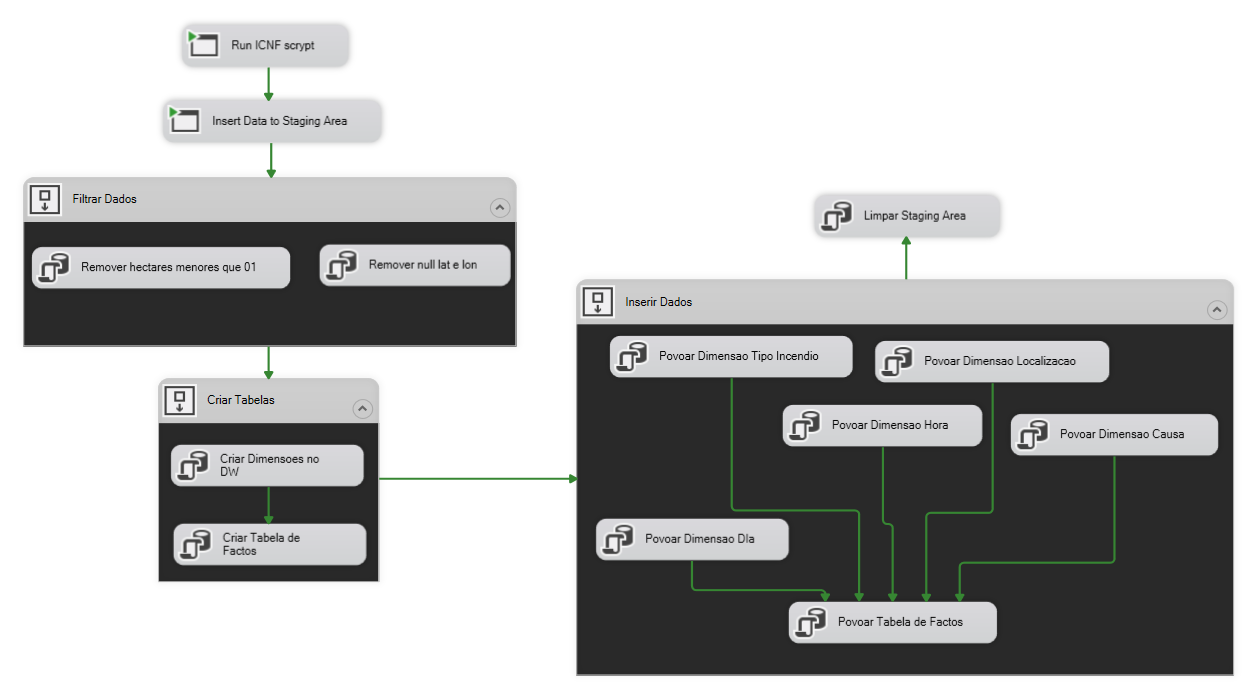
\includegraphics[width=0.9\linewidth]{imagens/ETL_incendios}
	\caption{Processo ETL para incêndios}
	\label{fig:etlIncendios}
\end{figure}

\subsection{Temperaturas}
No fluxo de ETL dos dados meteorológicos, o SSIS inicia a execução chamando um \textit{script} em \textit{Python} (via executável). Este \textit{script} consulta a tabela de factos dos incêndios para identificar os dias e locais exatos das ocorrências, extraindo apenas a meteorologia relevante e inserindo-a na \textit{Staging Area}.

Uma vez carregados os dados em \textit{Staging}, procede-se ao povoamento das dimensões e da tabela de factos no \textit{Data Warehouse}. Visto que os dados meteorológicos são recolhidos de forma direcionada (apenas para os dias/locais necessários) e provêm diretamente da API do \textit{Open-Meteo}, não é necessária a aplicação de filtros adicionais nesta fase.

Dado que este processo depende dos dados de localização e data dos fogos, a sua execução tem como precedência obrigatória a conclusão do processo ETL descrito na secção \ref{section:etlIncedios}.

\begin{figure}[htbp]
	\centering
	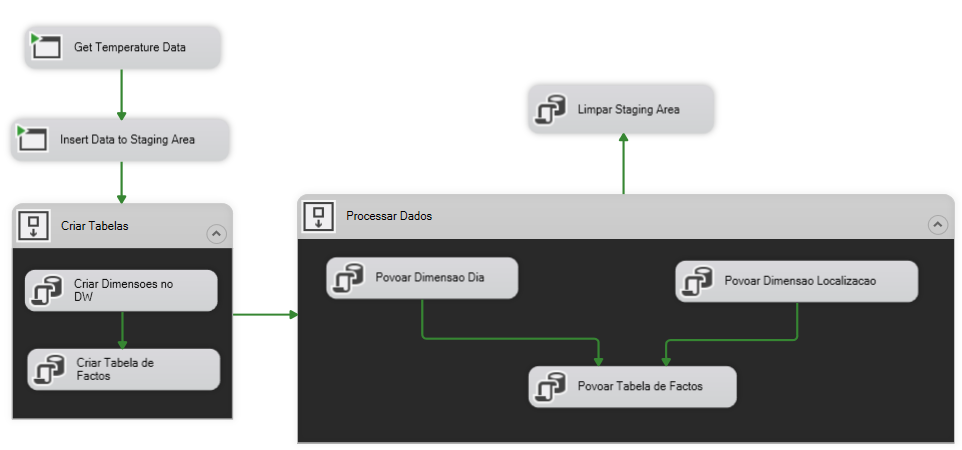
\includegraphics[width=0.9\linewidth]{imagens/etl_temperaturas}
	\caption{Processo ETL para temperaturas}
	\label{fig:etlTemperaturas}
\end{figure}

\subsection{Cobertura Mediática}
Neste fluxo, o executável responsável pela extração de notícias não foi integrado diretamente no pacote ETL principal. Isto deve-se ao facto de o processo incluir, para além da extração, uma etapa de enriquecimento de dados através de um modelo de \textit{Machine Learning}. Visto que esta etapa requer um tempo de processamento elevado, optou-se por desacoplá-la para simplificar a demonstração do processo de carga.

Portanto, para o correto funcionamento deste processo no SSIS, é pré-requisito a existência de um ficheiro JSON no diretório configurado, contendo os dados já processados pelo modelo. A partir desse ficheiro, o SSIS aciona um executável auxiliar para inserir os dados na \textit{Staging Area}. Com os dados carregados, o fluxo prossegue para alimentar todas as tabelas do respetivo esquema em estrela através de \textit{scripts} em T-SQL.

\begin{figure}[htbp]
	\centering
	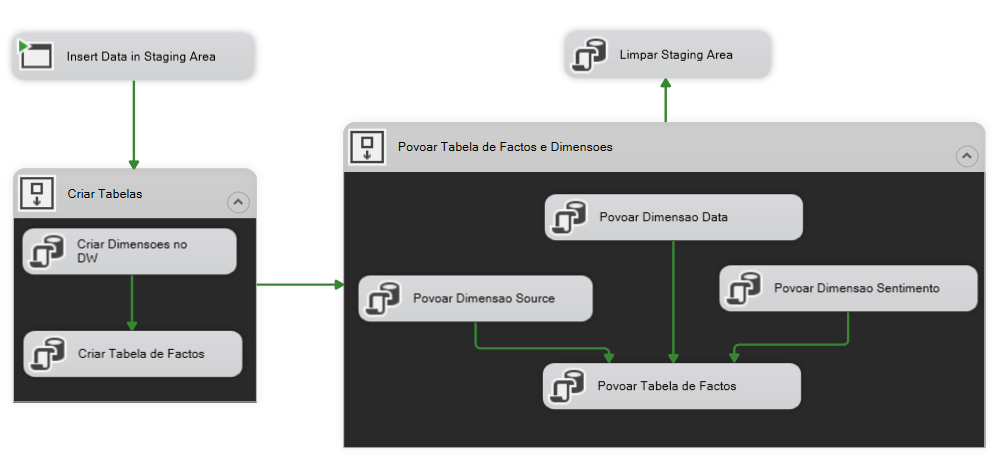
\includegraphics[width=0.9\linewidth]{imagens/etl_cobertura_mediatica}
	\caption{Processo ETL para cobertura mediática}
	\label{fig:etlCoberturaMediatica}
\end{figure}

\subsection{Vegetação}
À semelhança do verificado na cobertura mediática, a extração de dados do \textit{Google Earth Engine} (GEE) não foi integrada no fluxo automatizado do SSIS, devido à complexidade técnica de automatização da recolha nesta plataforma específica. Desta forma, o projeto SSIS foi configurado para ingerir ficheiros CSV previamente extraídos e depositados no diretório do projeto.

Foi estabelecida uma dependência funcional estrita para este processo: a sua execução ocorre obrigatoriamente após o processo ETL dos Incêndios. Esta precedência é necessária pois o carregamento dos dados de vegetação exige a consulta prévia à tabela de factos dos incêndios, garantindo assim a correta associação com a dimensão de localização e a integridade referencial do modelo.

Tal como nos restantes processos, eventuais falhas de inserção de registos resultam na geração de um ficheiro de \textit{log} de erros.

\begin{figure}[htbp]
	\centering
	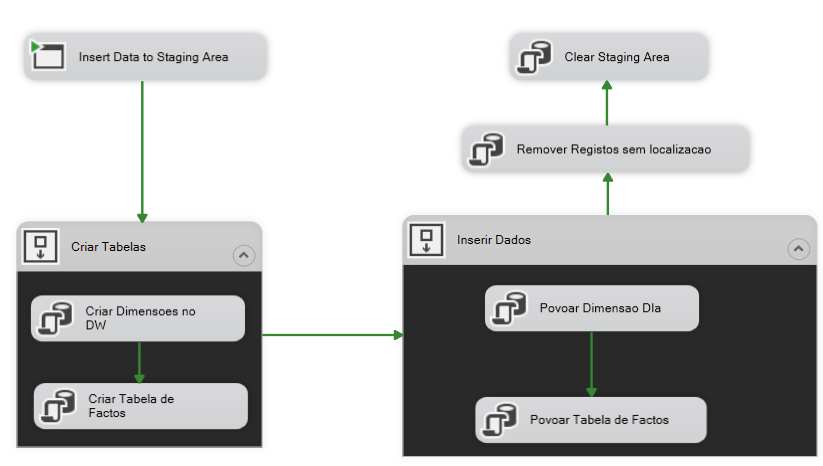
\includegraphics[width=0.7\linewidth]{imagens/etl_vegetacao}
	\caption{Processo ETL para vegetação}
	\label{fig:etlvegetacao}
\end{figure}